\documentclass{article}
\usepackage{graphicx}
\title{ECE 1895 - ASSIGNMENT 5 REPORT}
\author{Yinhao Qian}
\begin{document}
	\maketitle
	
	\section{SPICE Verification}
	There are going to be two versions of the spice simulation: one is for the actual PCB design and one is solely for testing purpose only. The reason I would have to create a separate ones for testing and PCB design is \textbf{I was unable to find capacitors with large values (more than 1 $\mu$F) in Benedum 1223}, so I have decided to replace all capacitors with values more than 1$\mu$F with 1$\mu$F. If everything goes well, the only changes should be the frequency of oscillations and nothing else. I'll demonstrate this is the case in the upcoming sections.
	
	\subsection{Version 1 - SPICE for PCB Design}
	For resistor designated with $ R909 $ and $ R501 $, I would simplify the circuit by combining them into a new resistor designated with $ R909R501 $, and I'll change simulate the circuit two times with each resistances. \newline
	\subsubsection{Schematics}
	\textbf{This is when 511 Ohm is used: }\newline
	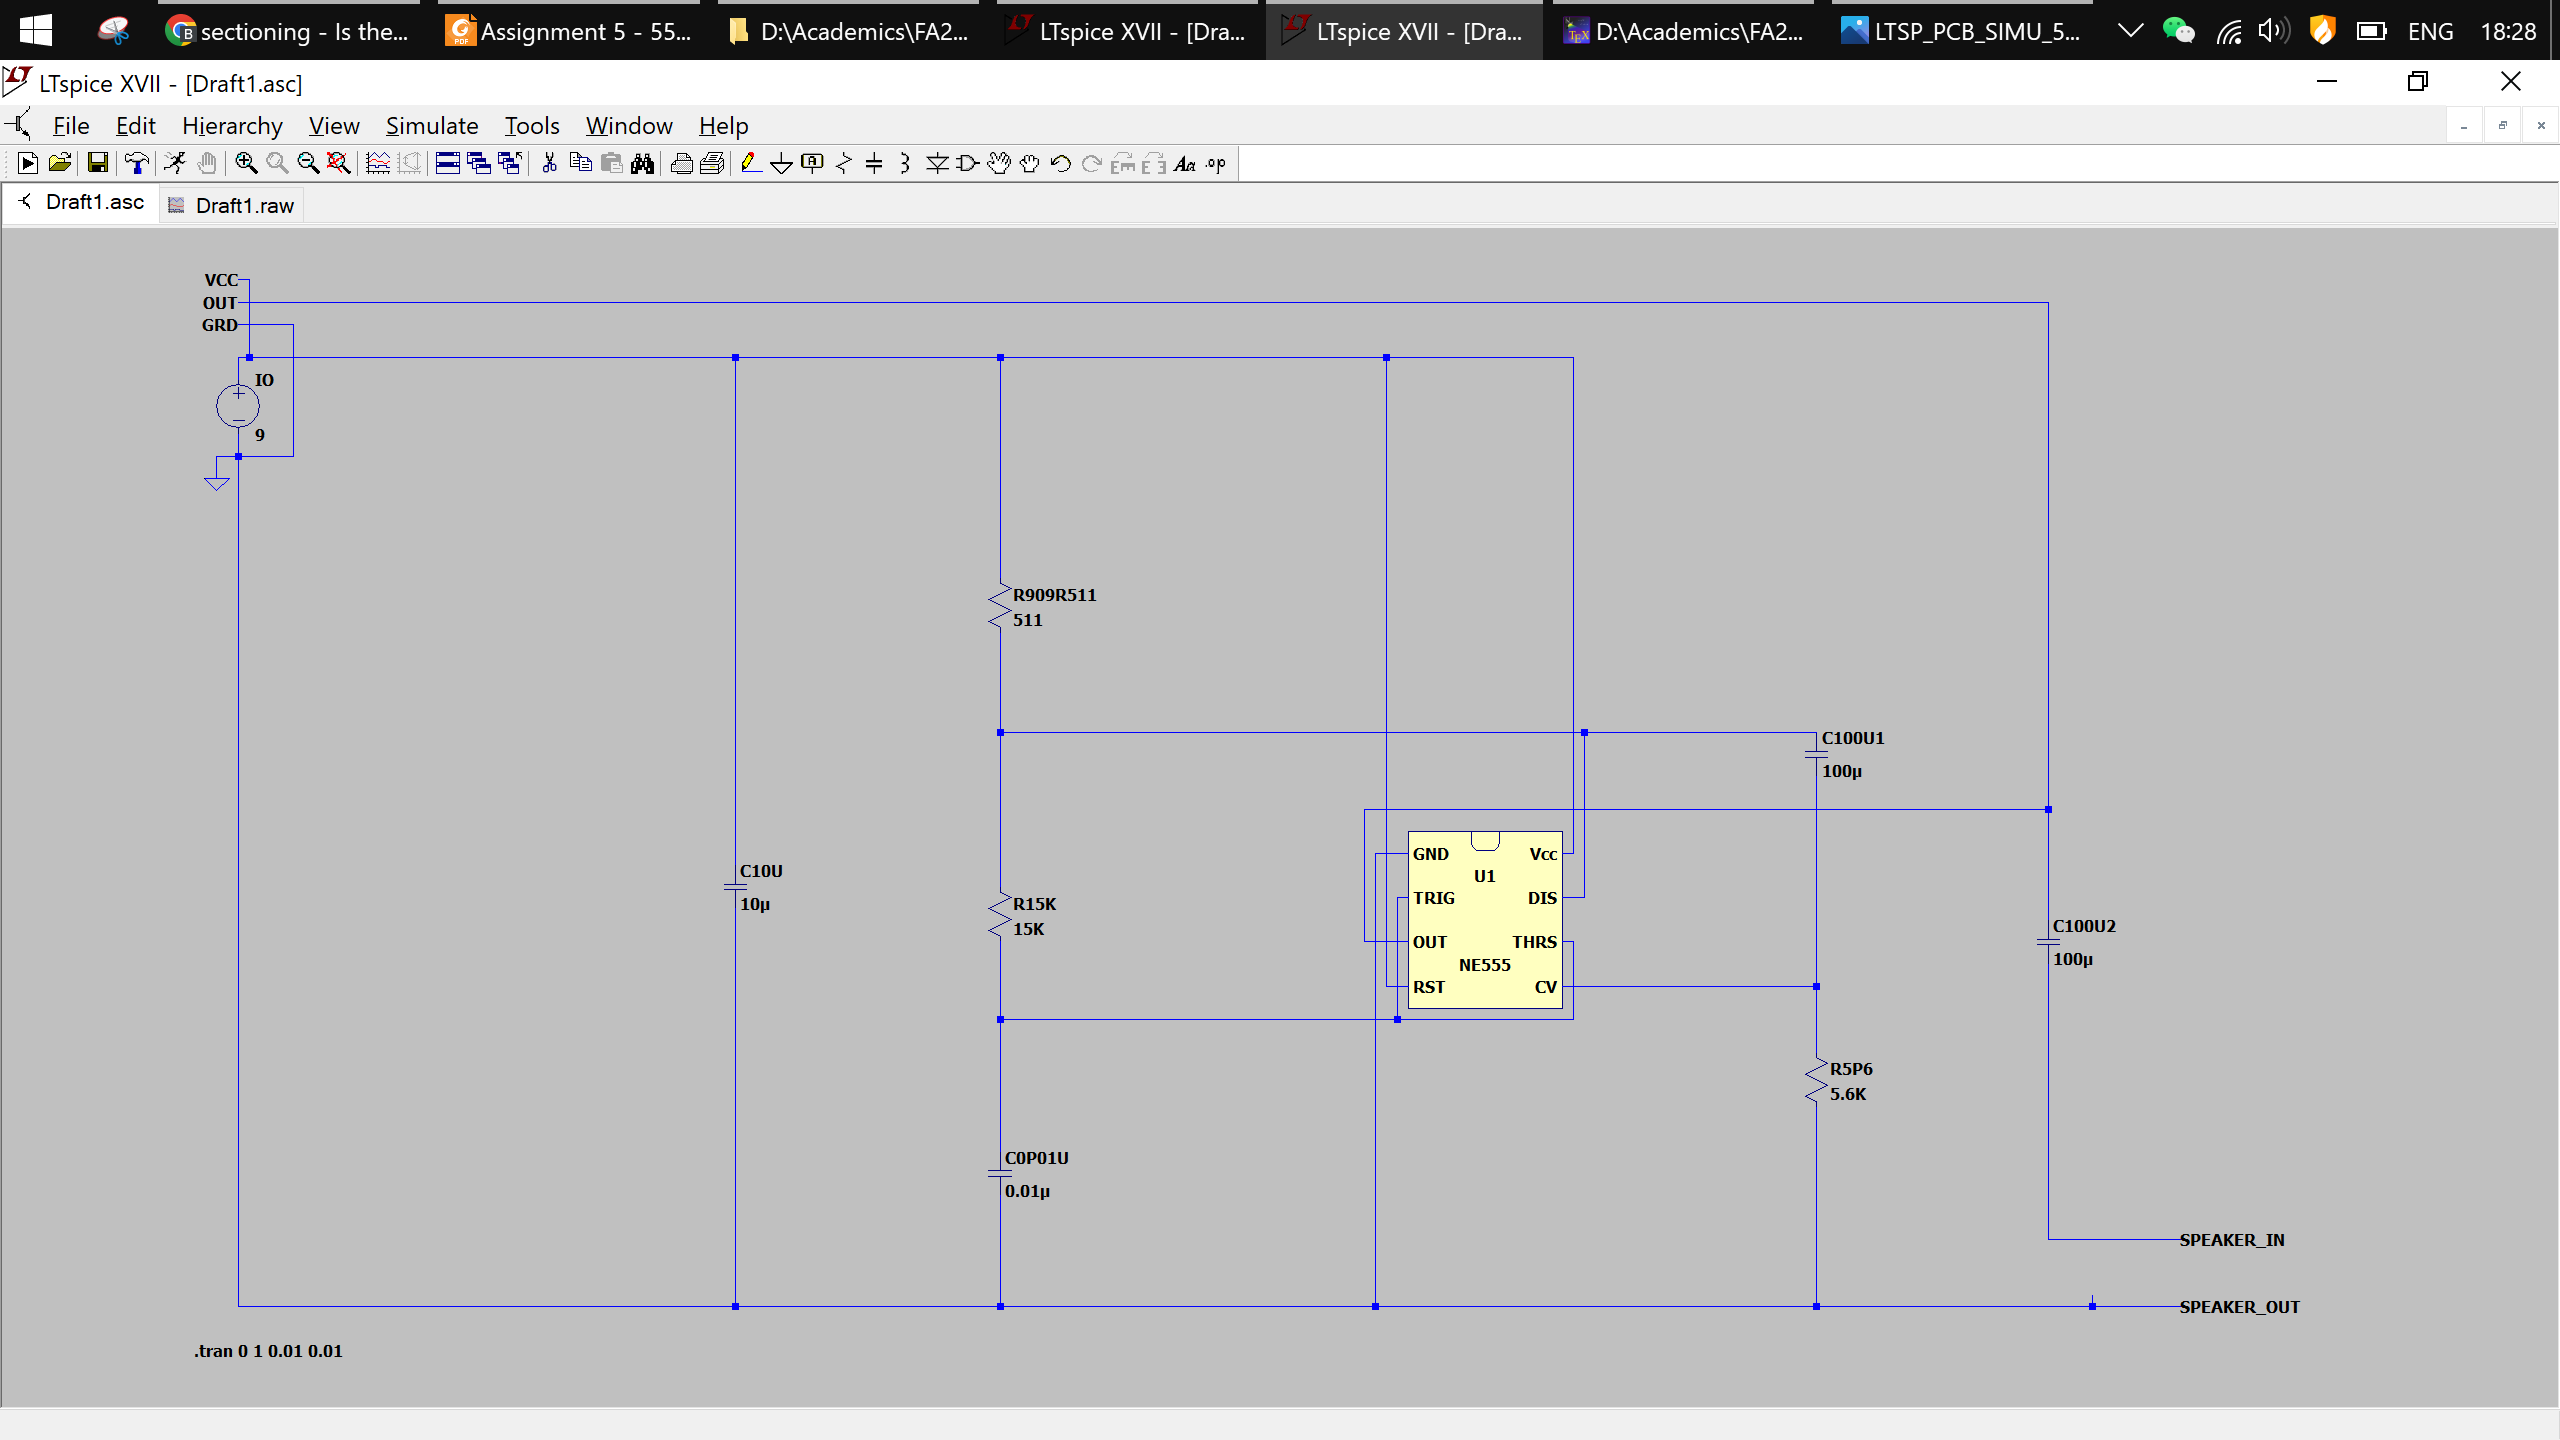
\includegraphics[width=\columnwidth]{LTSP_PCB_SCHE_511}
	\textbf{This is when 909 Ohm is used: }\newline
	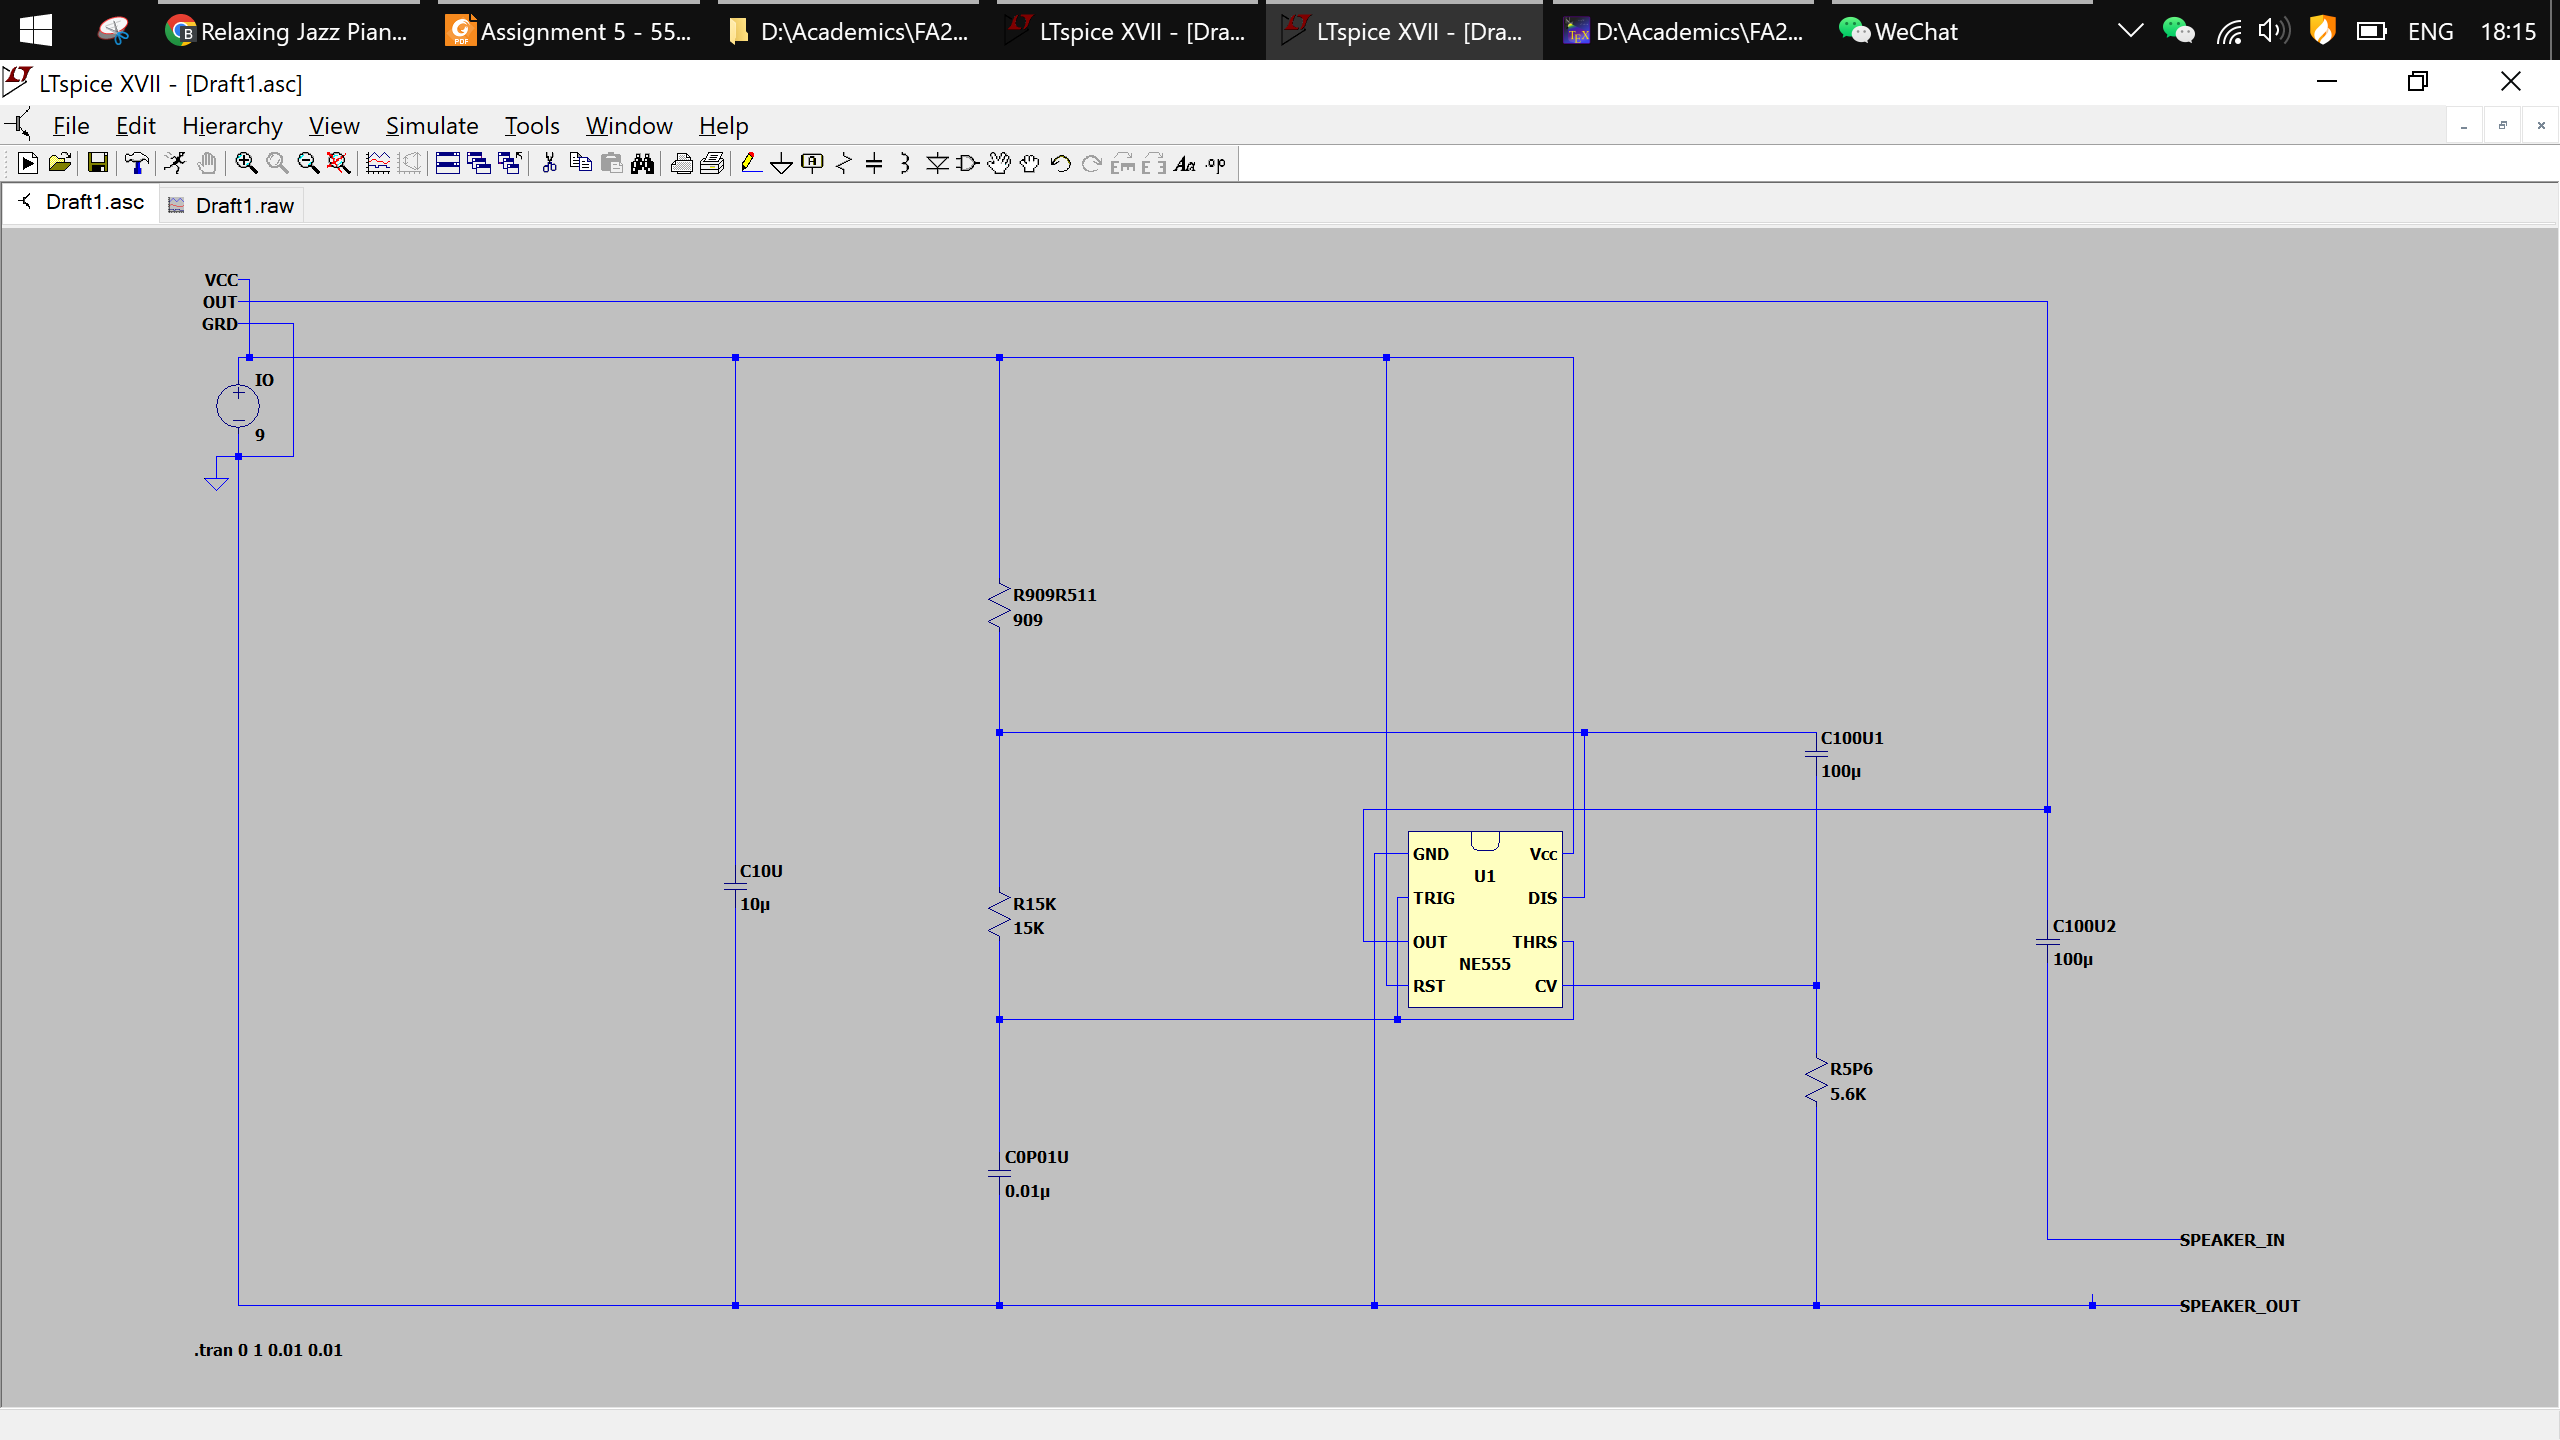
\includegraphics[width=\columnwidth]{LTSP_PCB_SCHE}
	No other changes are made except for the resistor values.
	\subsubsection{Simulation}
	\textbf{This is when 511 Ohm is used: }\newline
	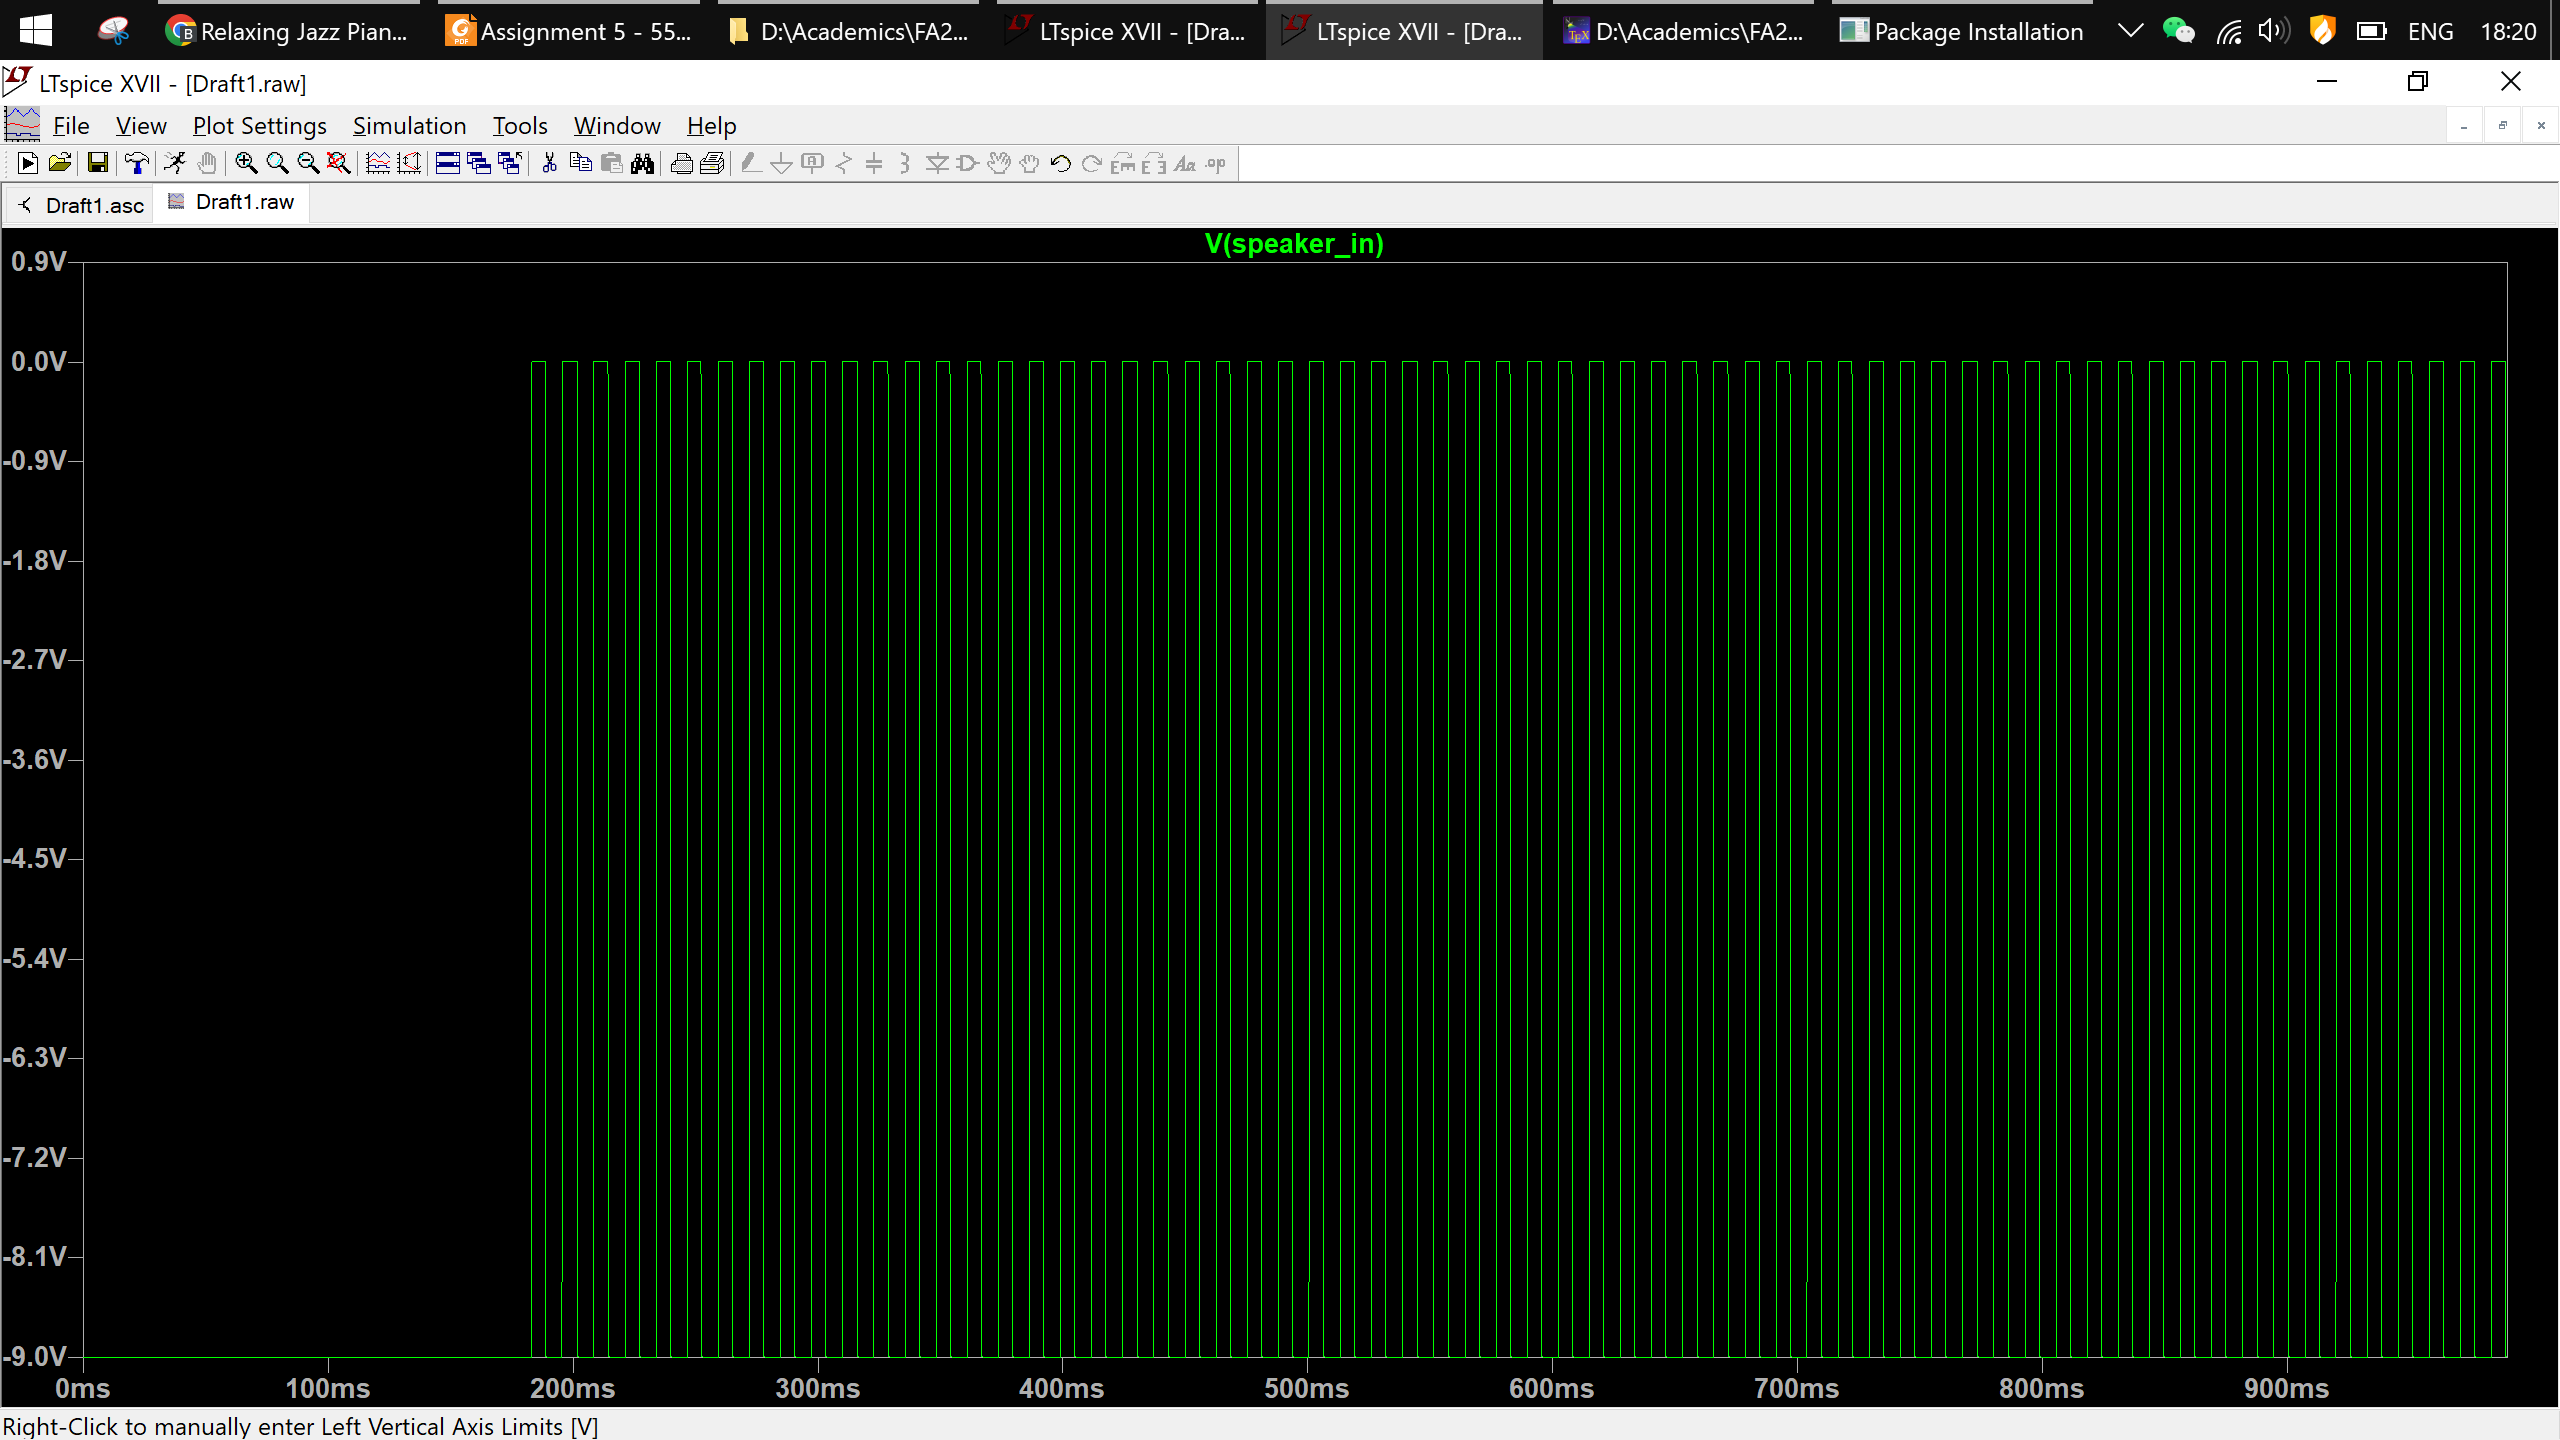
\includegraphics[width=\columnwidth]{LTSP_PCB_SIMU_511}
	\textbf{This is when 909 Ohm is used: }\newline
	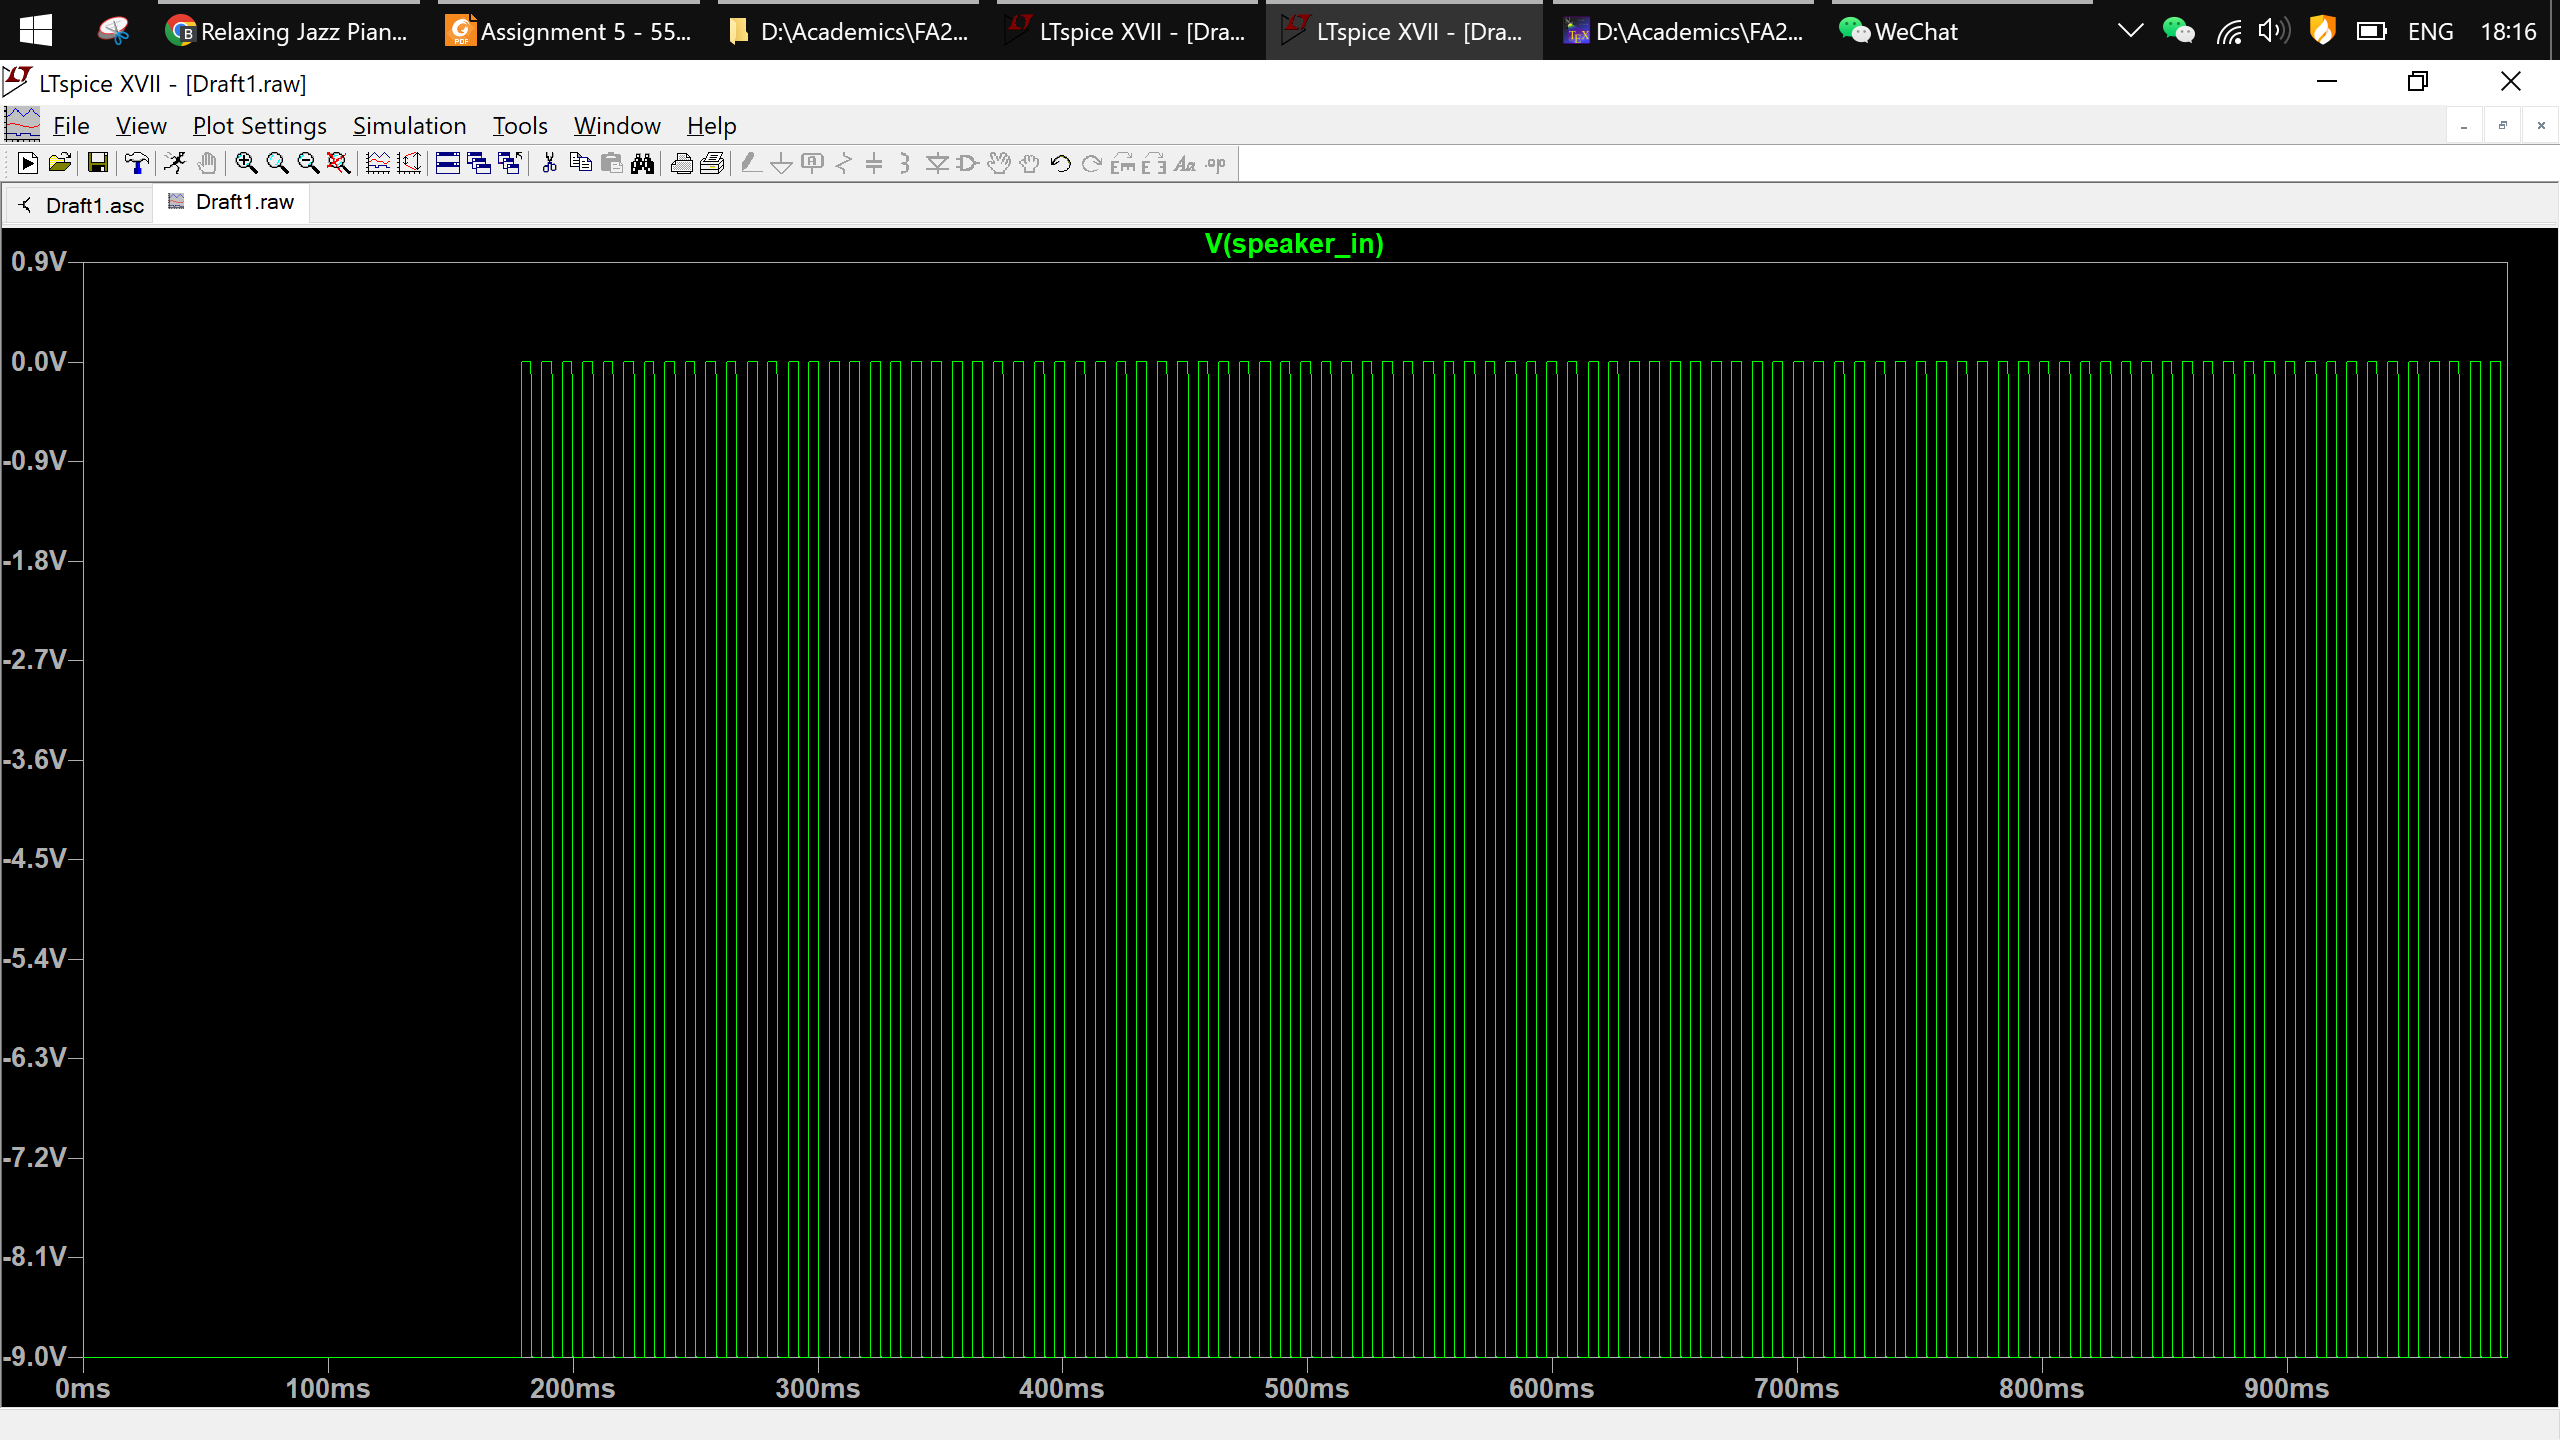
\includegraphics[width=\columnwidth]{LTSP_PCB_SIMU}
	An interesting observation here is that the resistance of $ R909R511 $ is \textbf{directly proportional} to the frequency of generated output.
	\subsection{Version 2 - SPICE for Breadboard Testing}
	For resistor designated with $ R909 $ and $ R501 $, I would simplify the circuit by combining them into a new resistor designated with $ R909R501 $, and I'll generalize the model by using a 1K-Ohm resistor, since it's the one I found in Benedum 1223. \newline
	\subsubsection{Schematics}
	Note that all capacitors with capacitance greater than $ 1\mu F $ are replaced with capacitors of $ 1\mu F $.\newline
	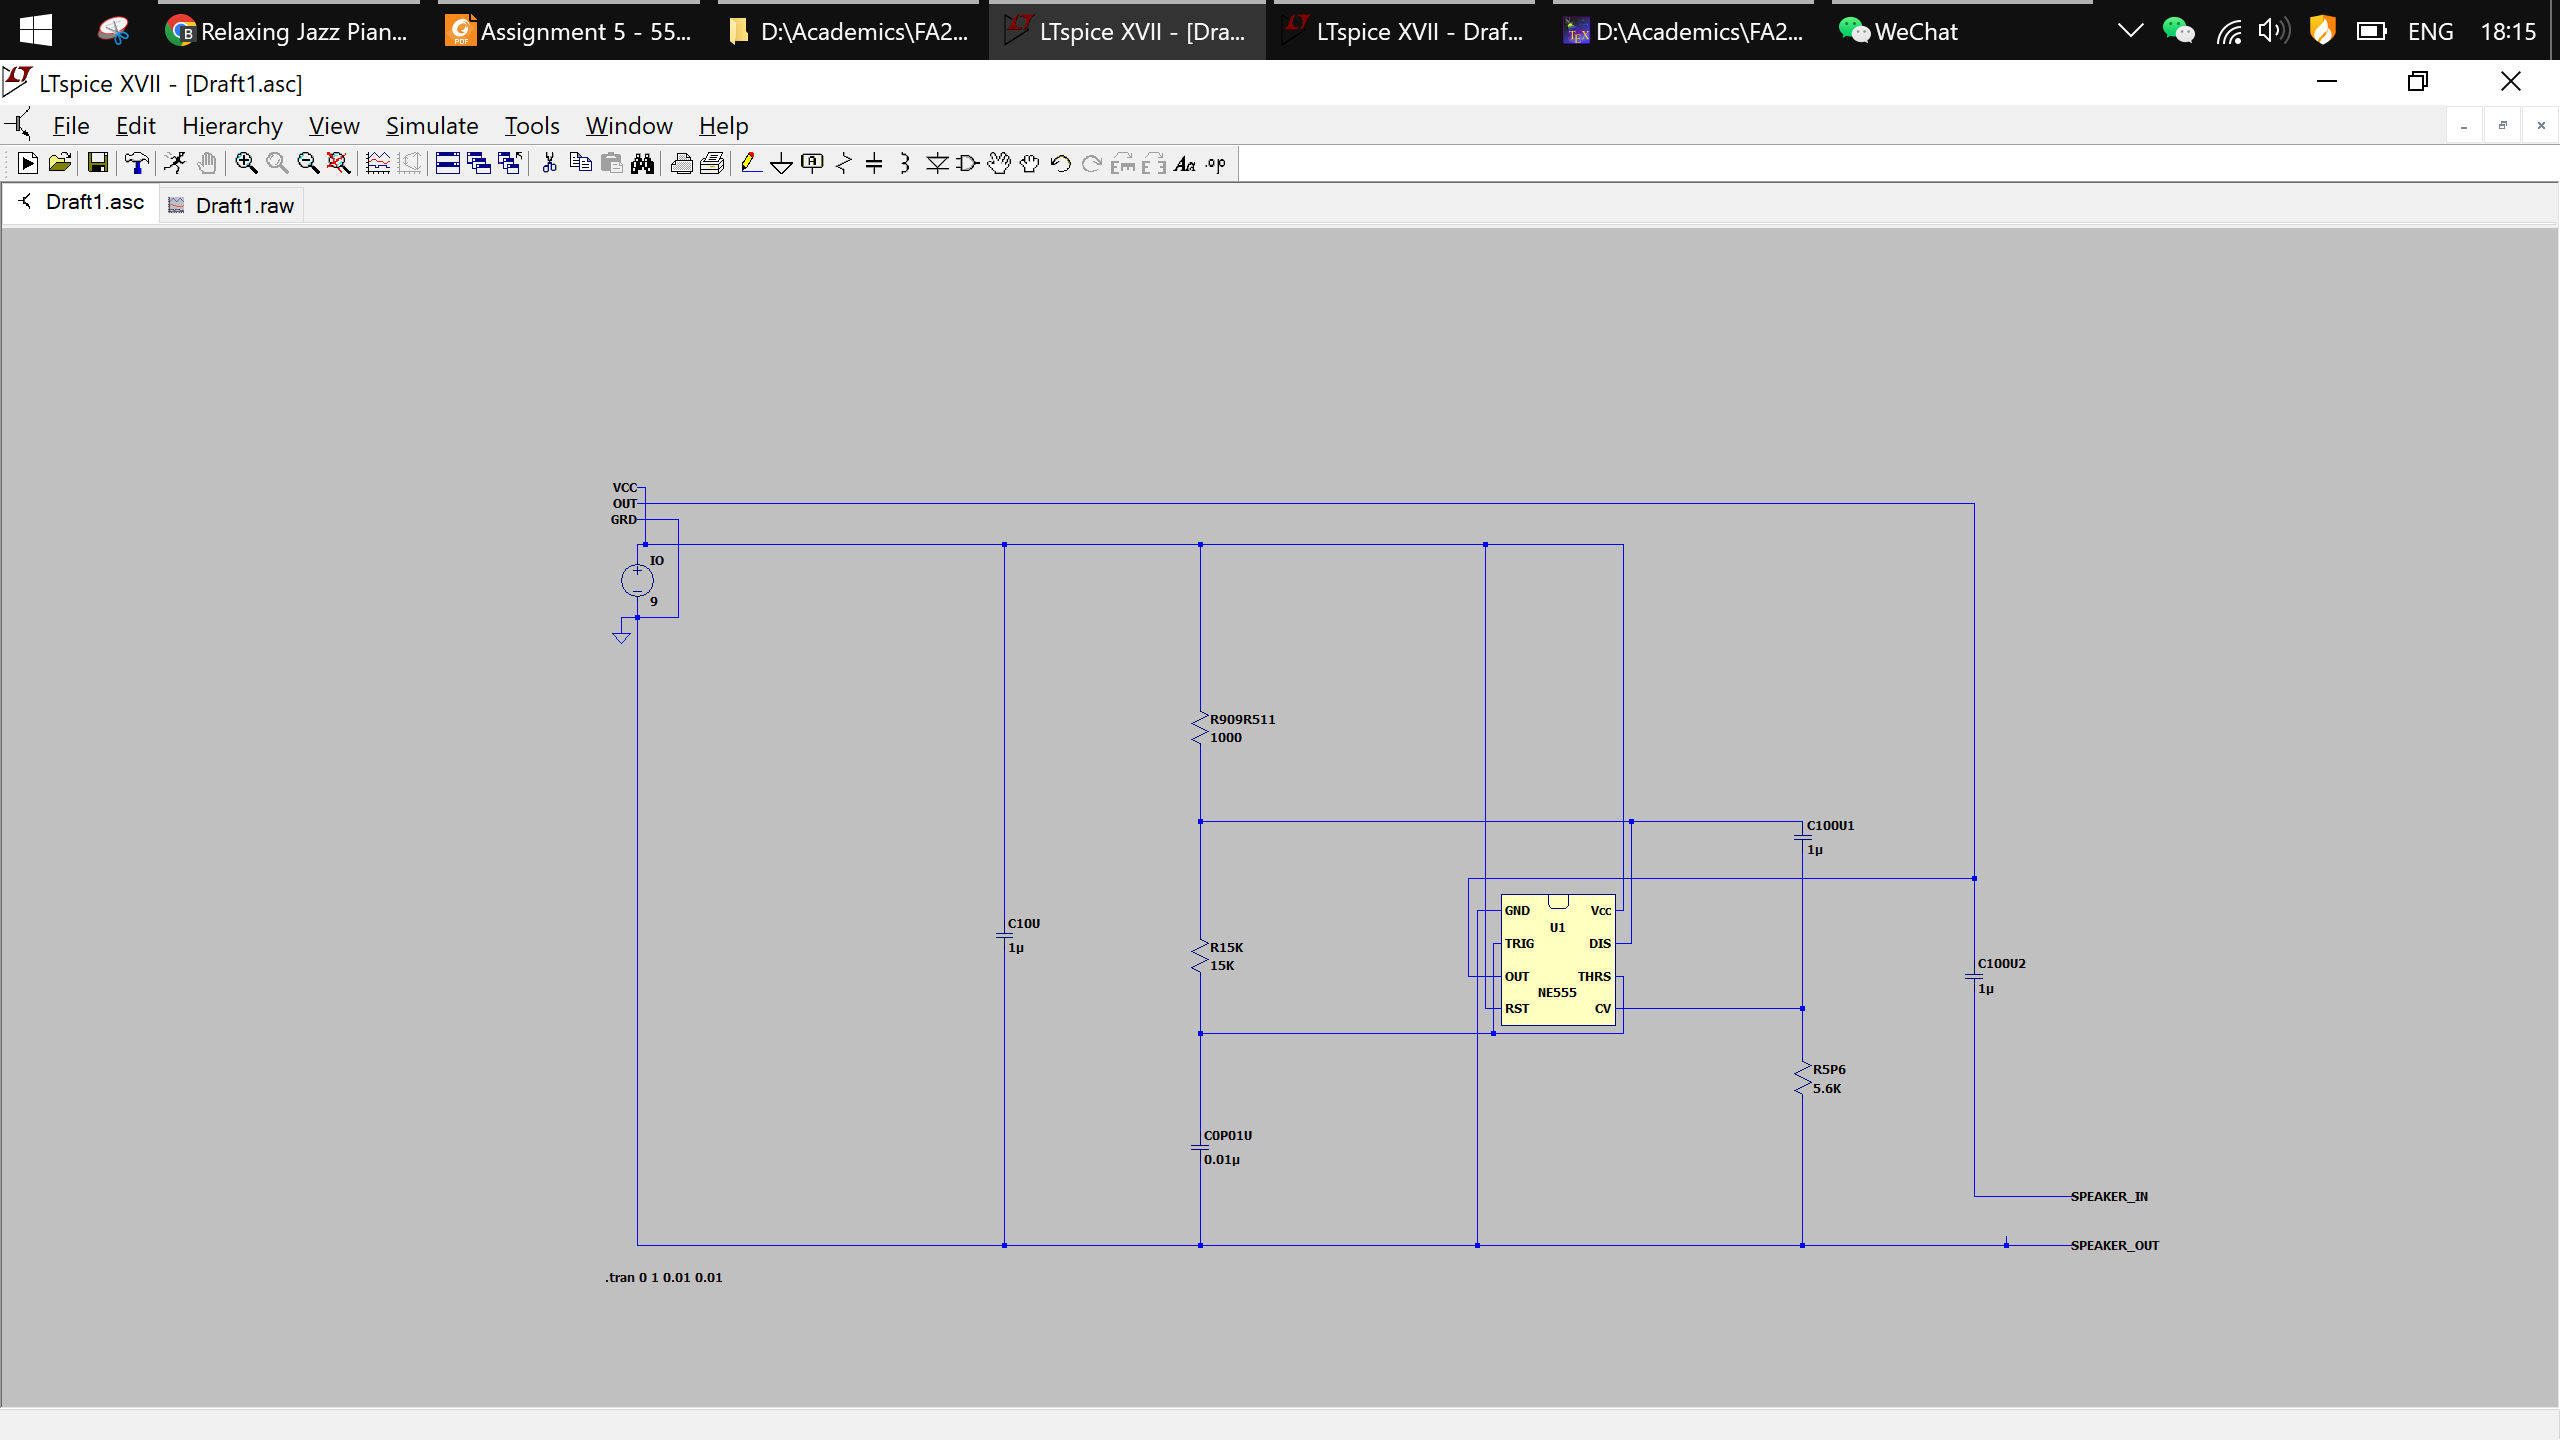
\includegraphics[width=\columnwidth]{LTSP_BREA_SCHE}
	\subsubsection{Simulation}
	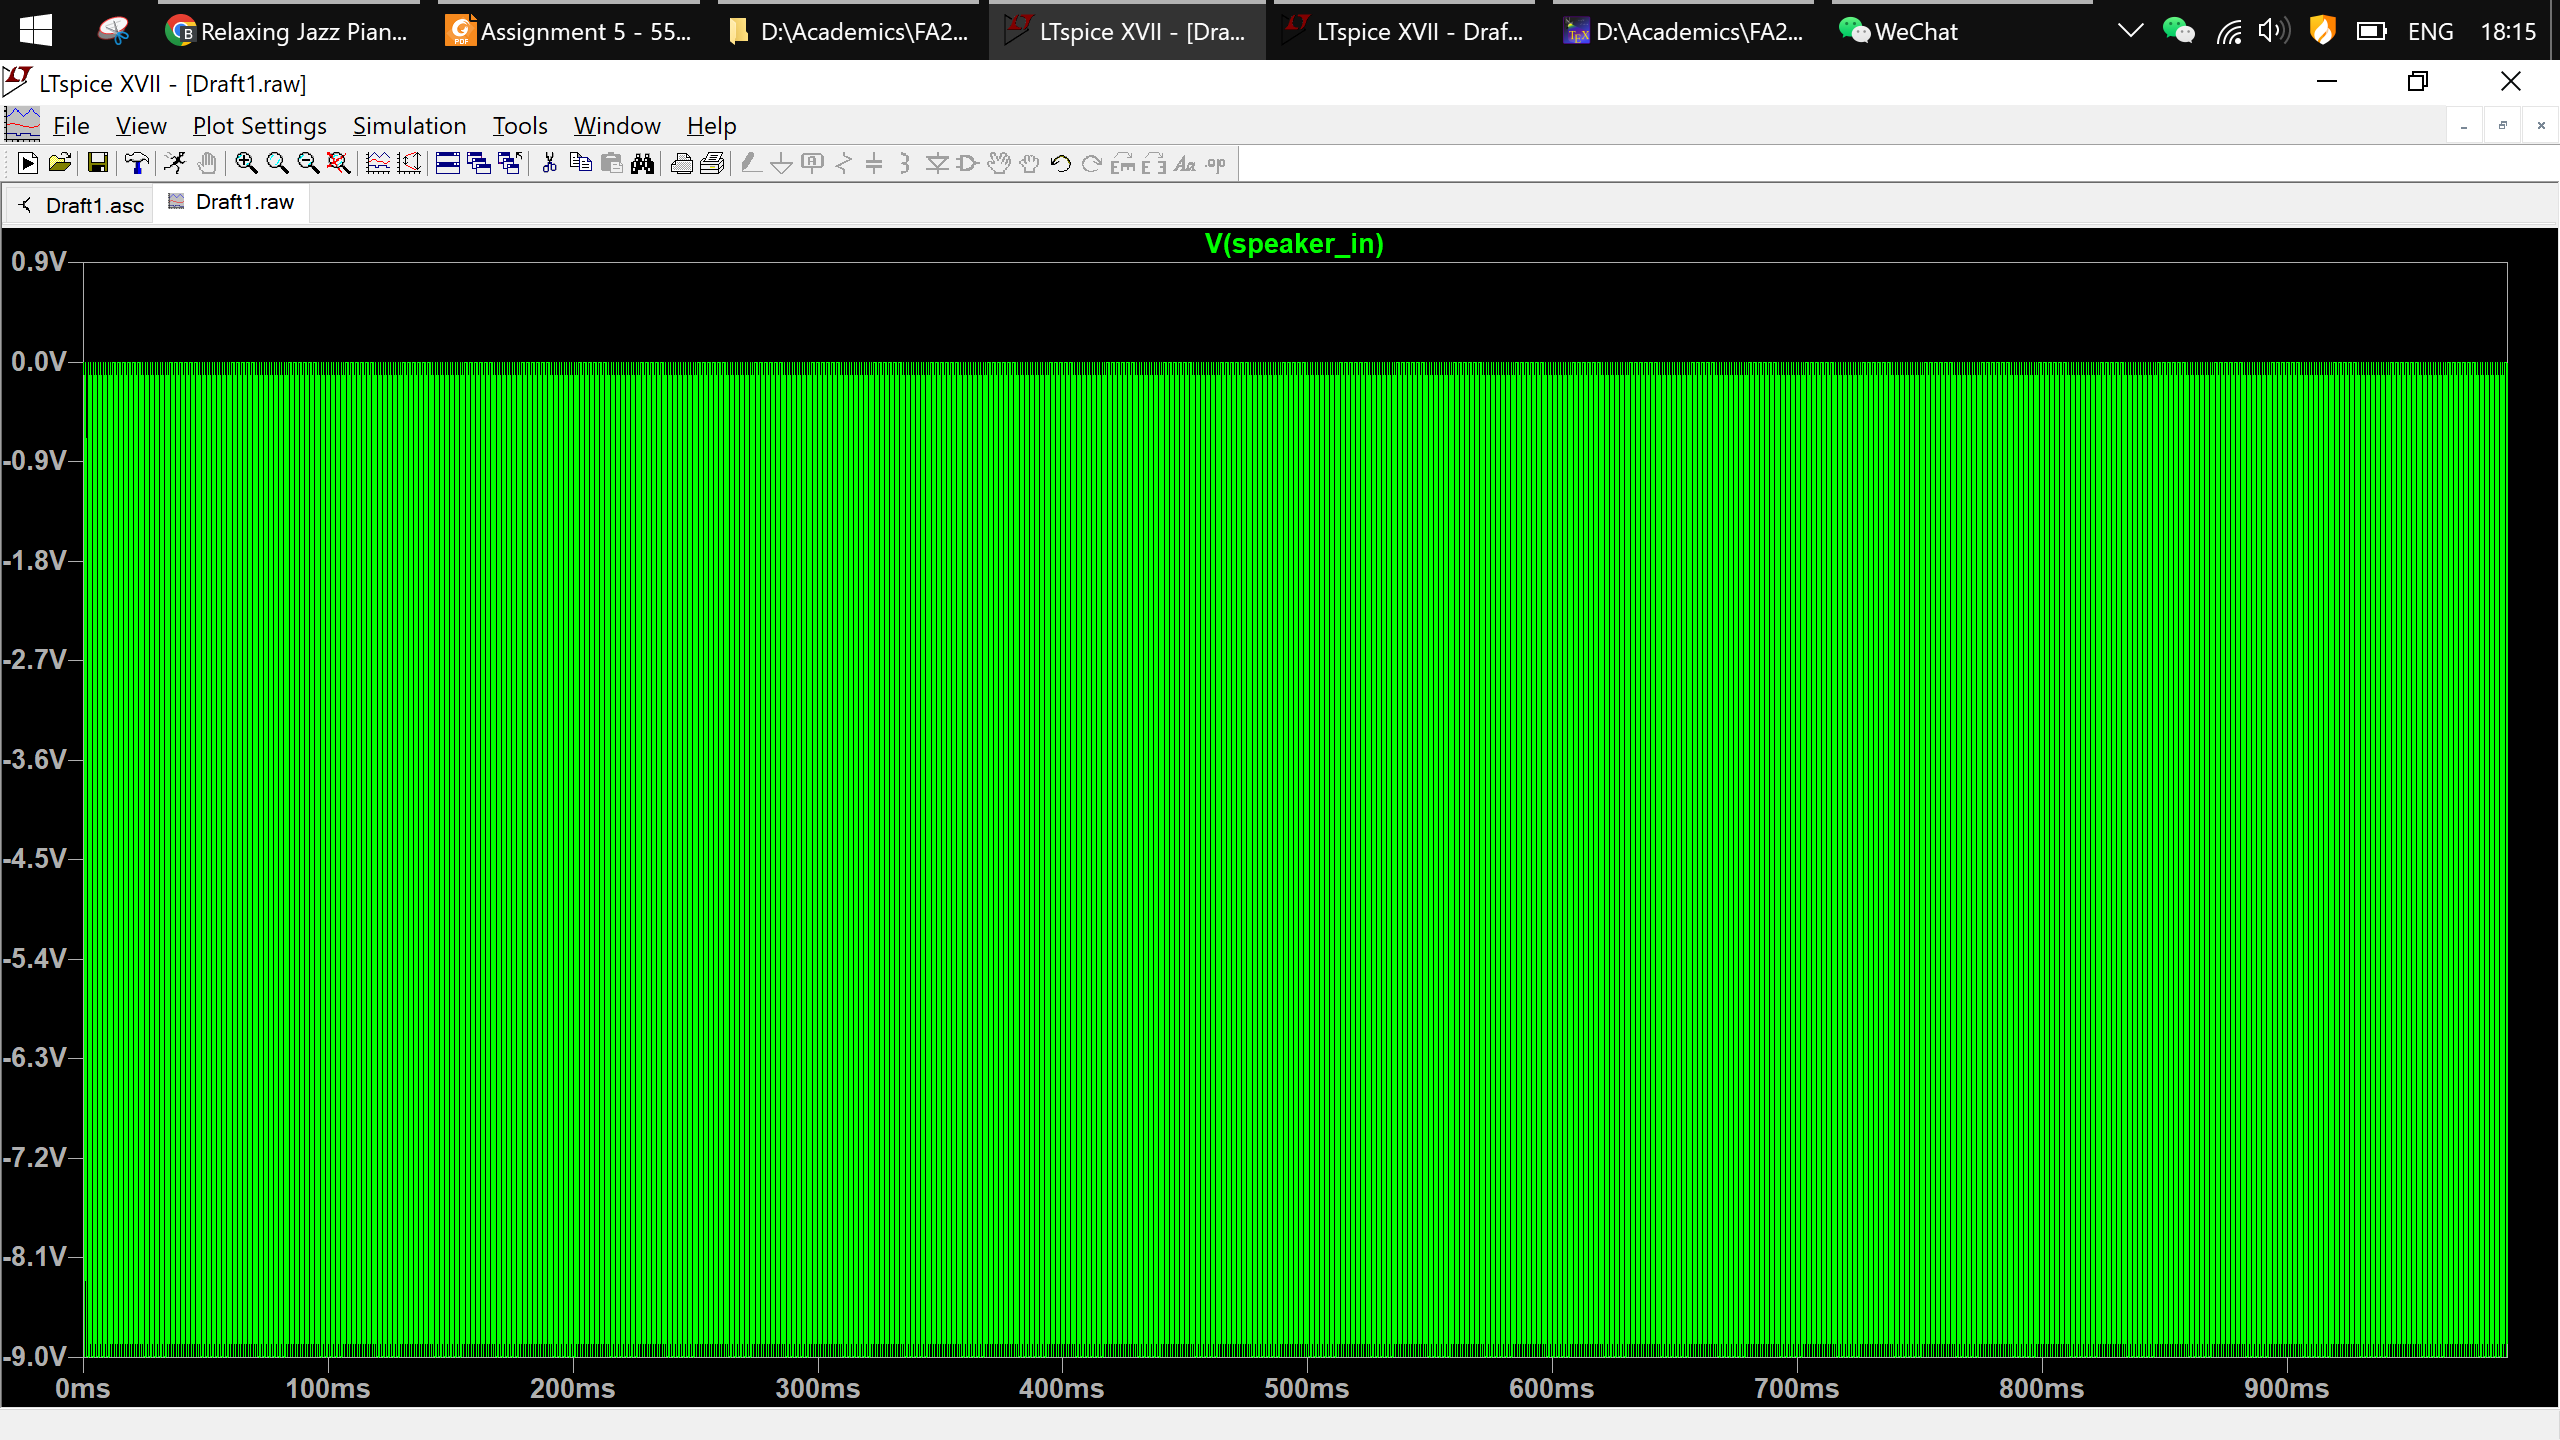
\includegraphics[width=\columnwidth]{LTSP_BREA_SIMU}
	We have noticed that the frequency does increased a lot, but as long as our measured voltage oscillates, we are good to go.
	\section{Breadboard Verification}
	I have connected wires and attempted to make matching circuits with reference to the schematics we made from previous section. Here's what it looks like on breadboard:\newline
	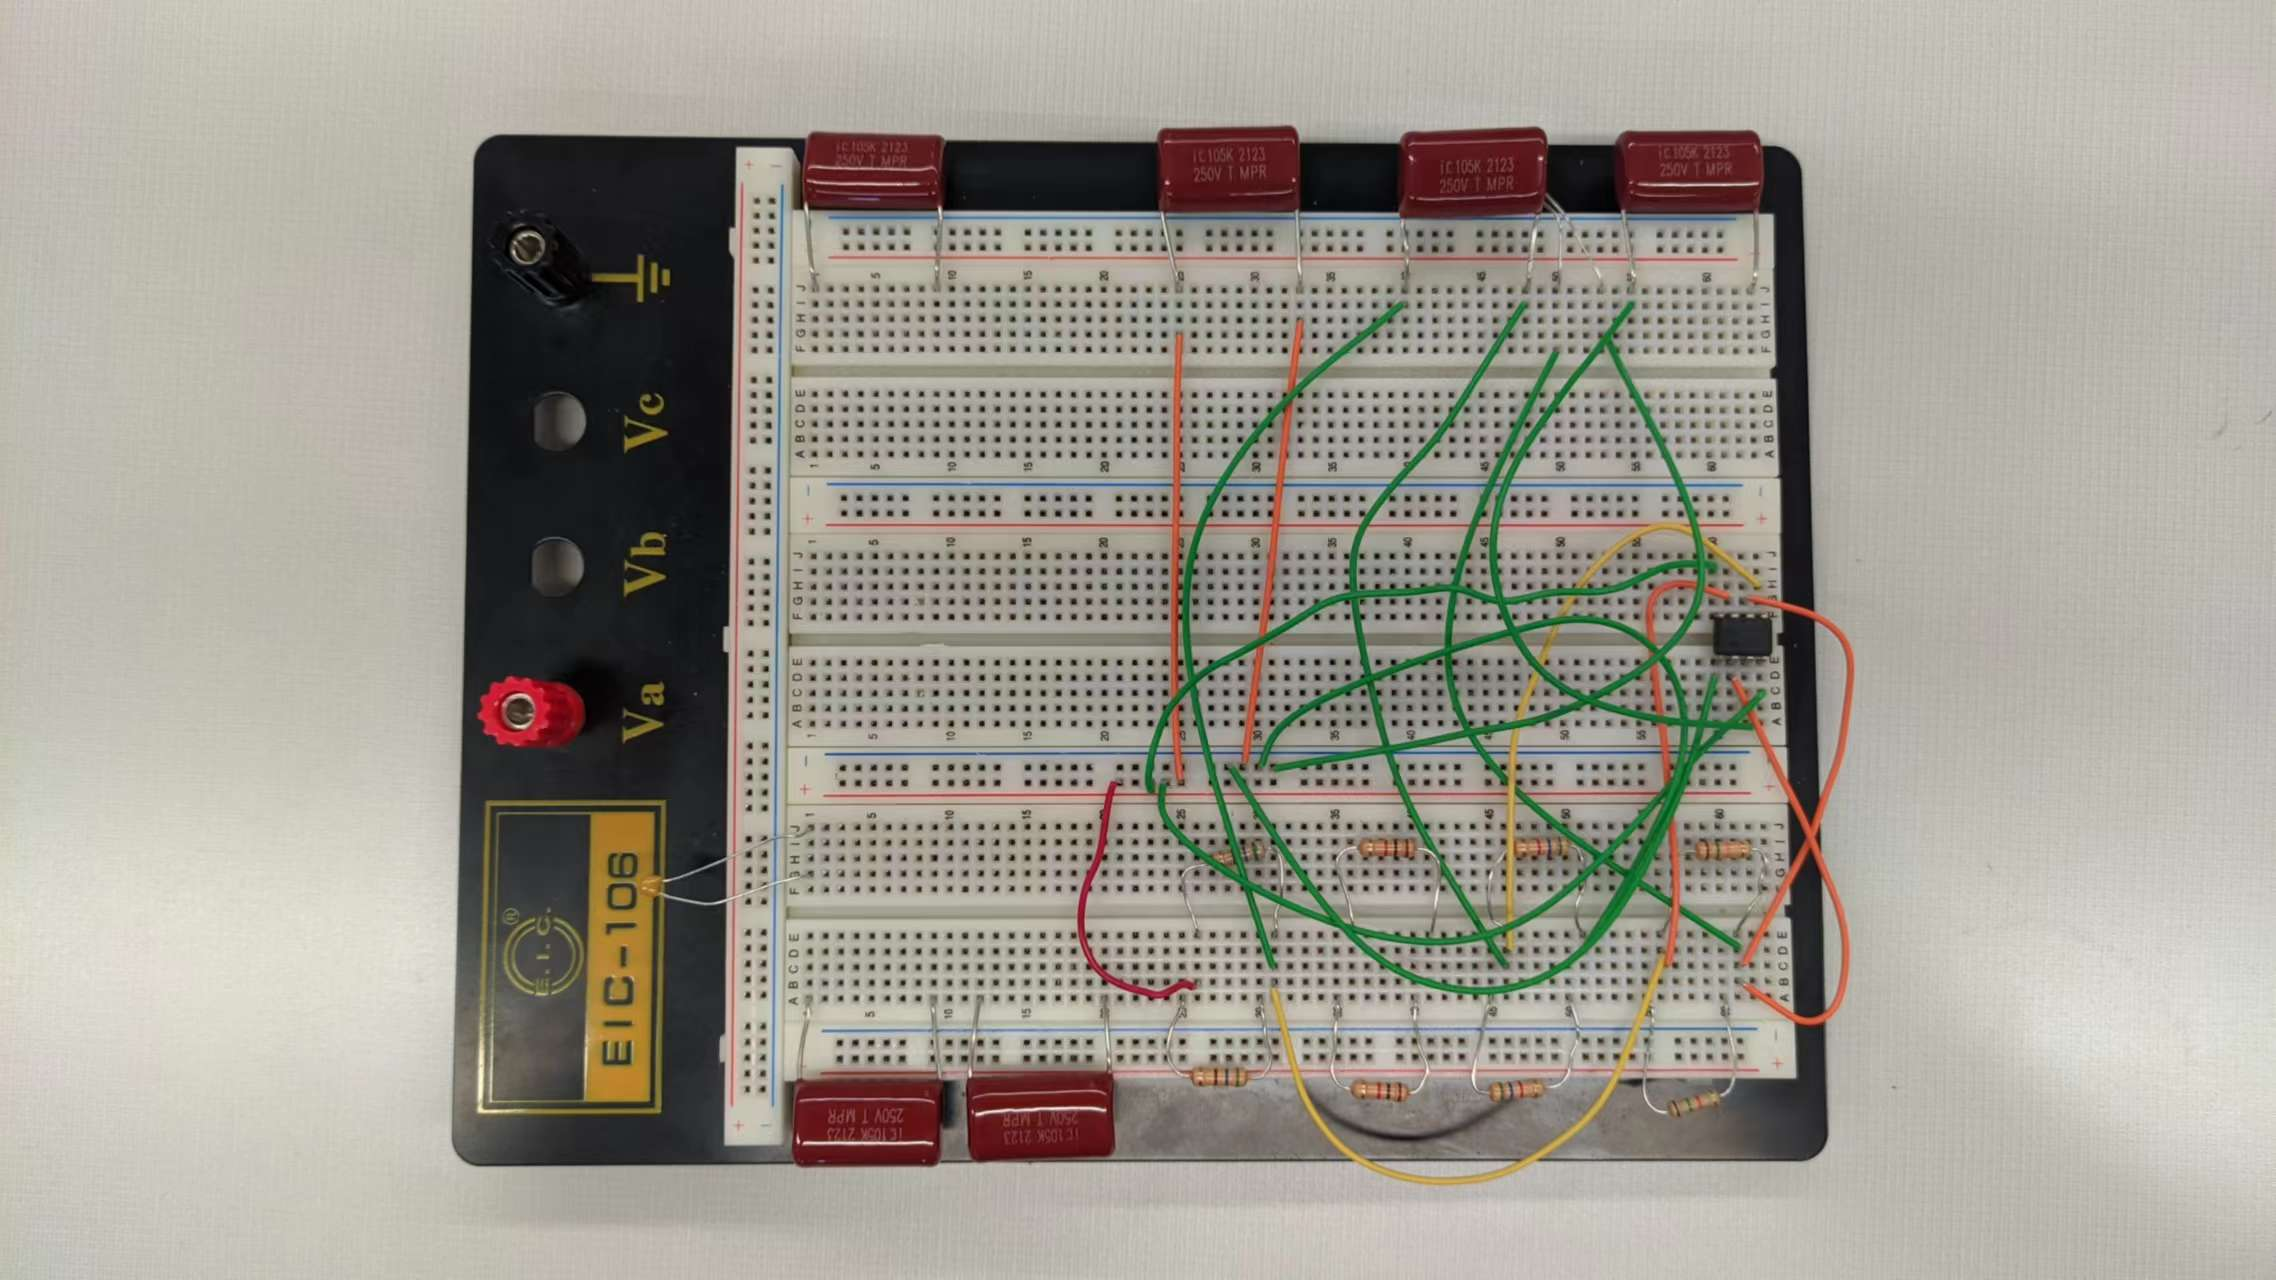
\includegraphics[width=\columnwidth]{BREA_SCHE}
	I understand it looks messy, that's why I hereby provide an visual aid with column/row numbers and wire-coloring matches.\newline
	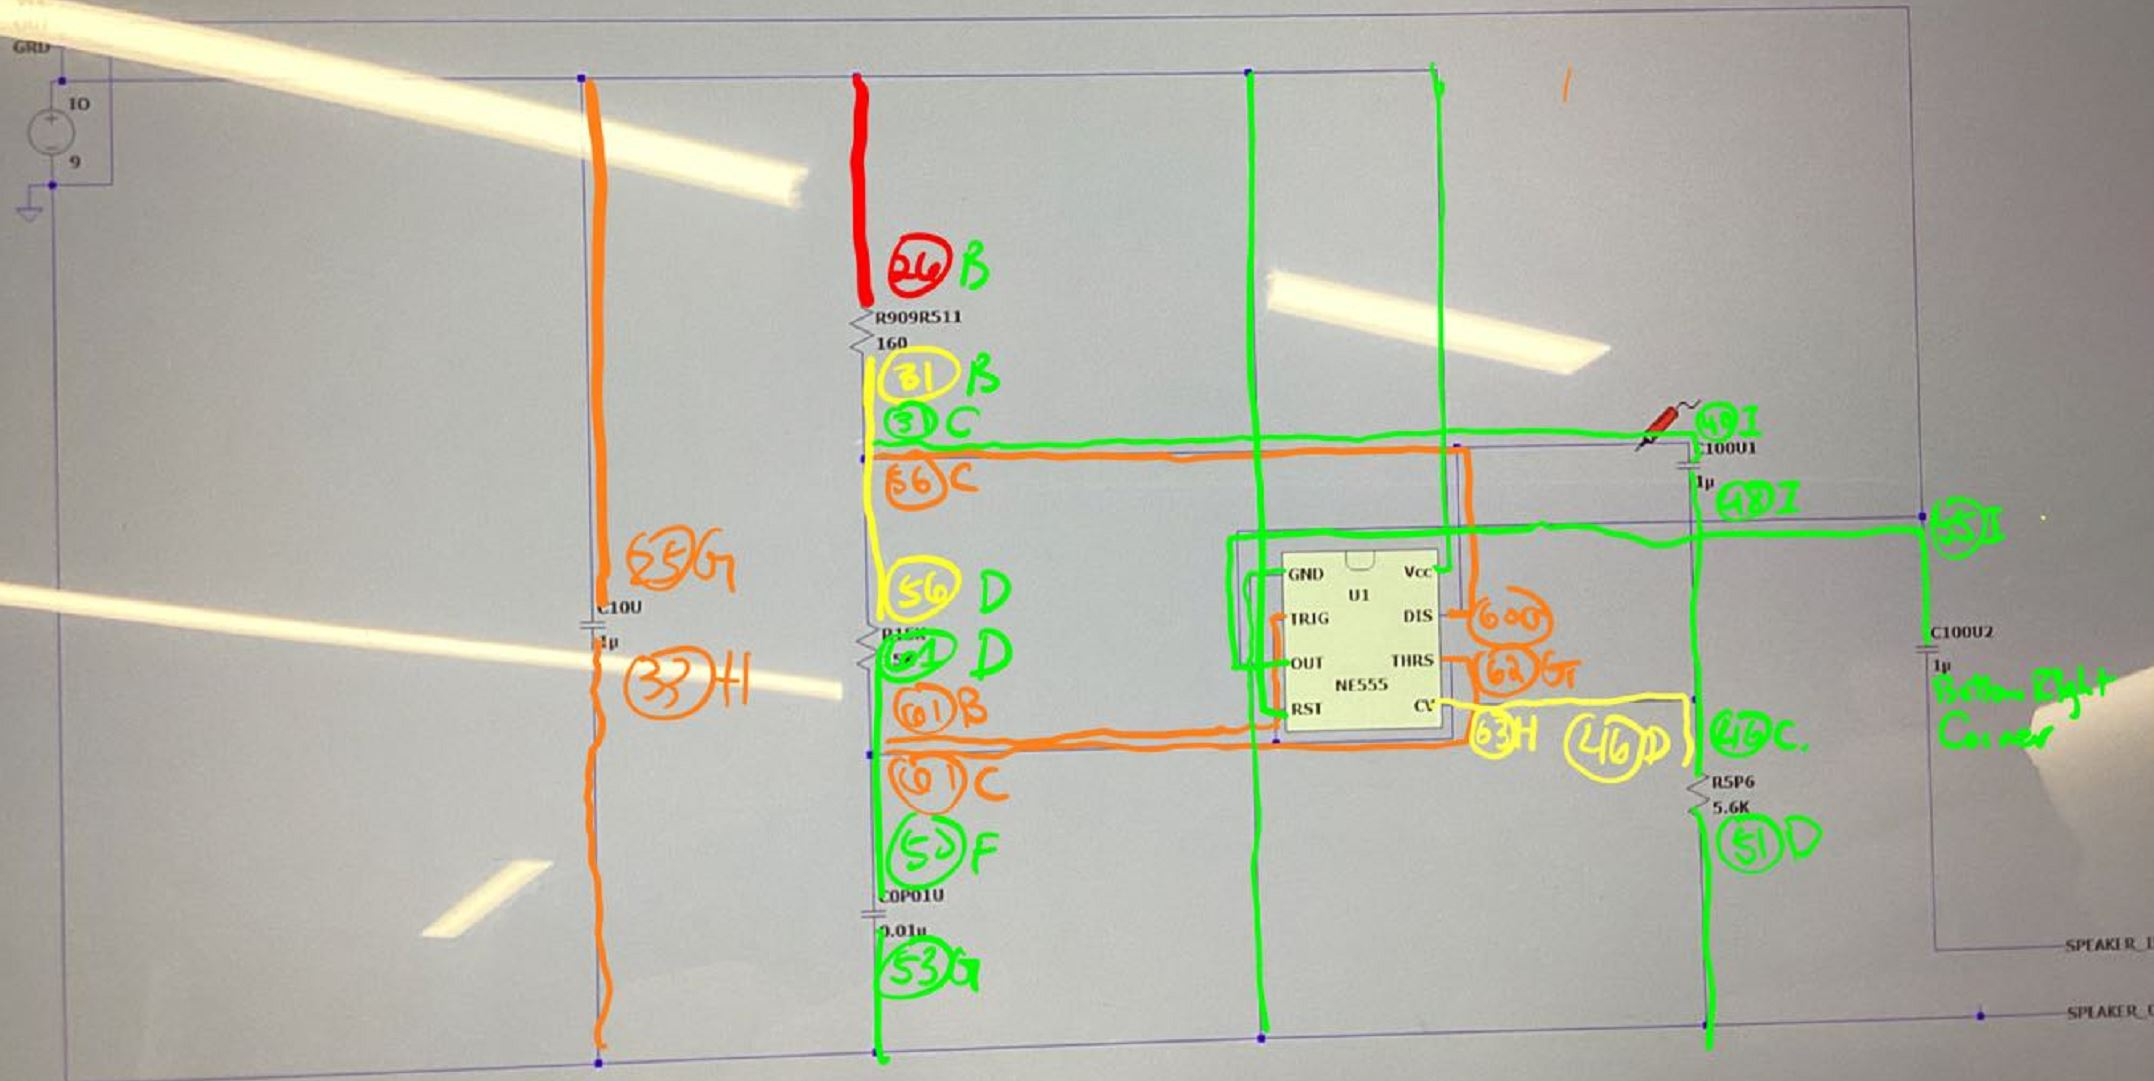
\includegraphics[width=\columnwidth]{LTSP_BREA_AID}

\end{document}